% !TeX program = xelatex

\PassOptionsToPackage{quiet}{fontspec}
\documentclass[12pt,a4paper,UTF8]{article}
\usepackage{thesis} % 格式控制
\usepackage{indentfirst}
\setlength{\parindent}{2em} % 控制首行缩进  
\addtolength{\parskip}{3pt} % 控制段落距离  
\onehalfspacing % 1.5倍行距  
\graphicspath{{./figures/}} % 指定图片所在文件夹  
\def\UrlBreaks{\do\/\do\-\do\_\do\.\do\?\do\&\do\=}
\Urlmuskip=0mu plus 2mu


\reporttitle{面向月球基地建设的材料运输运筹学优化方案}
\course{运筹学}
\studentname{曹航硕、吴天昊、陈禹成、邓凯坤、朱奕辰、{\CJKfontspec{Songti SC}康褀}}
\studentnamelines{曹航硕、吴天昊、陈禹成}{邓凯坤、朱奕辰、{\CJKfontspec{Songti SC}康褀}}
\studentid{}
\college{}
\major{}
\instructor{何衍}
\grade{}
\experimentdate{}
\makepagestyle{}{}




\begin{document}
\maketitlepage % 封面页

\maketoc    %目录页
\makeexperimentinfo % 正文首页页眉
\setcounter{section}{-1}
\section{题目、作者和摘要}

\subsection{题目}

面向月球基地建设的材料运输运筹学优化方案

\subsection{作者}

\begin{center}
\renewcommand{\arraystretch}{1.35}
\begin{tabular}{ccc}
\toprule
姓名 & 学号 & 专业 \\
\midrule
曹航硕 & 3240101938 & 机器人工程 \\
吴天昊 & 3240105556 & 机器人工程 \\
陈禹成 & 3240102176 & 机器人工程 \\
邓凯坤 & 3240105612 & 机器人工程 \\
朱奕辰 & 3240103075 & 机器人工程 \\
{\CJKfontspec{Songti SC}康褀} & 3240101043 & 机器人工程 \\
\bottomrule
\end{tabular}
\end{center}

\subsection{摘要}

本文围绕月球基地建设期的大规模材料运输问题展开研究。题目设定要求从地球向月球运输约 \(100\) Mt 建设材料，可选方式包括由三个 Galactic Harbours 组成的太空电梯系统和传统火箭运输系统。由于太空电梯具有低成本、低排放但年运力有限的特点，火箭具有高灵活性但成本和环境代价较高的特点，问题本质上是一个多目标运输资源配置问题。

本文首先计算仅使用太空电梯和仅使用火箭两类极端方案，作为成本、工期和环境影响的基准；随后建立以成本、工期和环境影响为目标的目标规划模型，并用混合整数规划和一维整数搜索进行求解与校验。在此基础上，进一步建立非完美工作状态模型，用可用率修正太空电梯和火箭的有效运输能力；最后建立扩展多时期发射场级模型，引入发射场环境敏感性、连续高频发射的非线性环境累积影响、10/60/30 建设运输节奏和火箭技术随时间进步等因素。

计算结果表明，纯太空电梯方案约需 \(186.22\) 年，工期过长；纯火箭方案需约 \(800000\) 次发射，成本和排放过高。因此，太空电梯与火箭结合的混合运输方案更合理。在完美工作状态下，成本+工期优先方案可在 50 年内完成，成本约 \(106.851\) trillion USD，排放约 \(0.841\) billion tCO2；非完美工作状态下，该方案需要增加火箭发射次数以弥补有效运力下降。综合考虑长期工程中的技术进步、施工节奏和环境调度，本文最终推荐扩展模型中的均衡方案：约 79 年完成运输，其中太空电梯承担 \(38.180\) Mt，火箭承担 \(61.820\) Mt，火箭发射约 \(504649\) 次，总成本约 \(74.295\) trillion USD，物理 CO2 排放约 \(0.701\) billion tCO2。

\clearpage
\section{前言}

\subsection{选题背景}

本报告选题改编自 2026 美国大学生数学建模竞赛（MCM）B 题：Creating a Moon Colony Using a Space Elevator System，题目网页为 \href{https://www.comap.org/membership/member-resources/item/creating-a-moon-colony-using-a-space-elevator-system}{COMAP 原题网页}。原题设定了一个面向 2050 年的未来工程场景：Moon Colony Management Agency 计划在月球上建设一个可容纳 100,000 人的 Moon Colony，并预计需要从地球向月球运输约 100,000,000 公吨建筑材料。题目同时给出两类主要运输方式：一类是由三个 Galactic Harbours 组成的 Space Elevator System，另一类是从地球现有火箭发射场出发的传统火箭运输[1]。

我们将原任务收敛为“探究月球基地建设期的材料运输方案”。我们的主要任务是：在 2050 年开始建设的条件下，比较仅使用太空电梯、仅使用传统火箭以及二者组合运输三类方案，并在成本、工期和环境影响之间寻找较优的材料运输方案。由于该问题同时涉及运输能力、发射次数、建设周期、环境排放、系统失效等多类因素，单纯依靠经验判断很难得到可解释的方案，因此需要借助运筹学建模方法进行定量分析。

\subsection{研究现状}

从现实背景看，月球基地建设和地月运输体系已经成为深空探测的重要方向。NASA Artemis 相关资料已经把月球基地、月面货运和长期驻留作为持续推进的方向[12][13]。现阶段较成熟的工程路径仍以火箭发射为主，其优势是技术路线清晰、发射场体系已有基础，但缺点也十分明显：单位运输成本高、发射次数需求巨大、环境影响和发射组织压力不可忽视。对于 100,000,000 公吨级别的建设材料运输任务，若完全依靠传统火箭，发射次数将达到极高数量级，运输组织和环境代价都会迅速放大。

太空电梯系统则代表另一类更具长期基础设施属性的运输方式。题目设定中的 Space Elevator System 使用 Galactic Harbour 将货物由地面提升至高轨位置，再通过较低燃料需求的方式转运至月球。已有太空电梯经济性研究认为，成熟太空电梯有可能显著降低单位入轨运输成本[2][3][4]。与火箭相比，太空电梯具有单位运输成本低、环境排放较小、长期稳定运行潜力大的优点；但其年运力受到系统规模限制，若只依靠电梯运输，建设周期会明显拉长。因此，单一运输方式都存在明显短板：火箭快但昂贵且污染高，电梯清洁且便宜但周期长。更符合实际工程决策的问题，是如何在两类运输方式之间进行组合，并根据不同决策偏好调整方案。

从运筹学角度看，该问题具有典型的多目标资源配置特征。它既包含运输问题中的运量分配思想，也包含整数规划中的火箭发射次数决策，还需要用目标规划处理成本、时间和环境三类目标之间的冲突。在进一步考虑非完美运行和发射场环境差异时，模型又会扩展出可用率修正、敏感性分析和非线性环境影响等内容。因此，本题不是简单的代入计算，而是一个适合用运筹学方法逐层抽象、逐步求解和进行方案比较的综合优化问题。

\subsection{研究意义}

本研究的意义首先在于把一个宏大的未来工程问题转化为可计算、可比较、可解释的优化模型。月球基地建设所需材料规模巨大，任何运输方式的单位成本、年运力或环境参数发生变化，都会在总成本、总工期和总排放上产生数量级影响。通过建立目标规划模型，可以明确不同决策偏好下的最优方案，而不是只给出单一结论。

其次，本研究能够体现运筹学课程中“建模—求解—评价”的完整思想。我们先用极端方案计算形成基准，再建立电梯和火箭混合运输的目标规划模型，随后讨论非完美运行条件下方案的稳定性，并进一步引入建设节奏、技术进步和发射场环境敏感性等扩展因素。这样的处理方式既保留了问题的现实复杂性，又避免模型一开始就过度复杂，便于解释每一层假设给结果带来的影响。

最后，本研究也具有较强的工程决策启发意义。对于长期基础设施建设问题，最低成本方案、最快完成方案和最低环境影响方案往往并不一致。通过对多种权重情景和模型扩展结果进行比较，可以帮助决策者理解：在不同政策目标下，太空电梯和火箭各自应承担怎样的运输比例，非完美运行会使方案发生多大偏移，以及更细致的发射场调度是否能降低环境代价。由此得到的结论不仅服务于本题设定，也能体现运筹学在大型工程规划、资源分配和多目标决策中的实际价值。

\begin{center}
    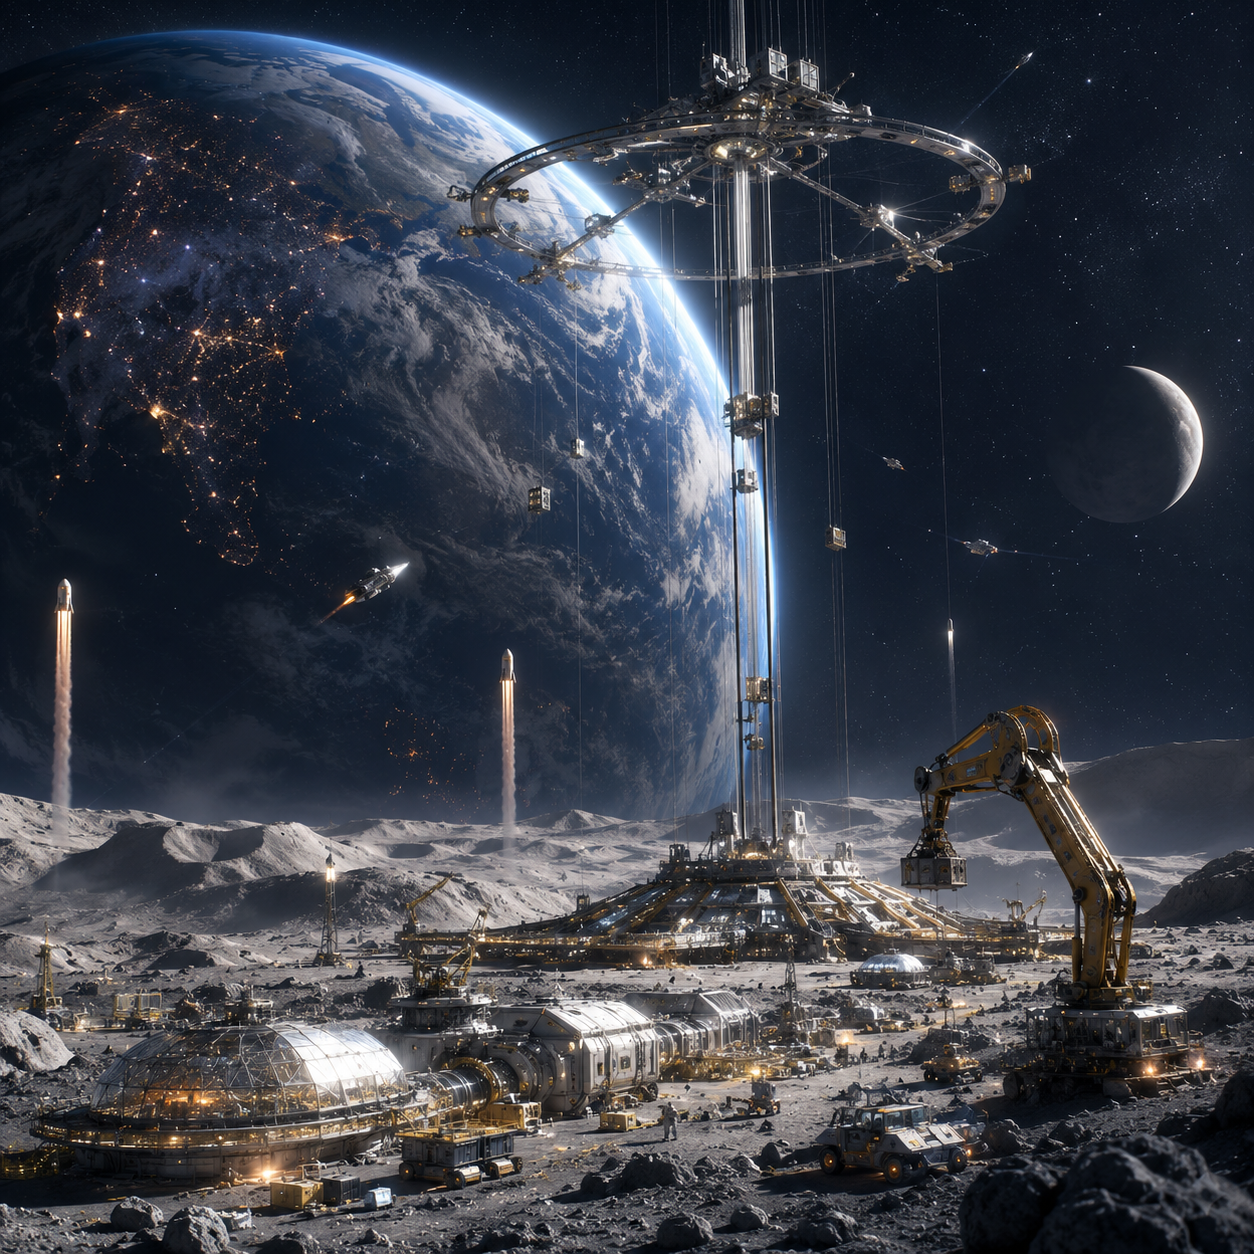
\includegraphics[width=0.68\textwidth]{figures/ChatGPT Image 2026年6月9日 16_56_07.png}
\end{center}

\clearpage
\section{问题描述}

\subsection{实际问题}

本题面对的是一个超大规模地月材料运输规划问题。按照原题设定，Moon Colony Management Agency 计划在 2050 年以后建设可容纳 100,000 人的月球基地，建设期需要从地球向月球运输约 \(100,000,000\) 公吨材料。可选运输方式主要有两类：一是 Space Elevator System，即由三个 Galactic Harbours 组成的太空电梯系统；二是从地球现有发射场发射的传统火箭系统。

原题对运输系统给出了若干关键条件。Space Elevator System 的最终配置包含三个 Galactic Harbours，理想情况下沿赤道相隔 \(120^\circ\) 分布；每个 Galactic Harbour 包含 Earth Port、两根长度为 \(100000\) 公里的 Tethers 和两个 Apex Anchors，并能够把货物提升至 GEO 及更远位置。题目给出的单个 Galactic Harbour 年运输能力为 \(179000\) 公吨/年，因此本文按三个 Galactic Harbours 同时投入使用计算，太空电梯系统年总运力为 \(537000\) 公吨/年[1]。

传统火箭方面，原题列出了 10 个可选发射场，包括 Alaska、California、Texas、Florida、Virginia、Kazakhstan、French Guiana、Satish Dhawan Space Centre、Taiyuan Satellite Launch Center 和 Mahia Peninsula。题目还假设到 2050 年，先进 Falcon Heavy 火箭可将 \(100\)--\(150\) 公吨有效载荷送达月球[1]。基础模型中，我们取中间值 \(125\) 公吨/次作为主值，并参考 Falcon Heavy 公开资料和 NASA 发射服务合同标定火箭能力与发射成本[7][8][9]。发射场位置与环境敏感性参数没有全部放入正文，详细列于附录\ref{app:sites}。

两类运输方式的优缺点并不相同。太空电梯系统单位运输成本较低、单位排放较小，但年运输能力有限，若单独承担全部材料运输，建设周期会过长。传统火箭运输速度更灵活，可以通过增加发射次数压缩工期，但其单次运输成本高、发射次数巨大，并会带来更高的环境排放。因此，本题不能简单归结为“选择电梯”或“选择火箭”，而应研究两类运输方式之间的合理组合。

从决策角度看，我们需要回答三个层次的问题。第一，在运输系统理想运行时，仅使用太空电梯、仅使用火箭和二者混合使用分别会产生怎样的成本、工期和环境影响。第二，当太空电梯或火箭系统并非完美运行时，原有最优方案会发生多大变化。第三，在更现实的建设情景下，如果进一步考虑建设阶段节奏、发射场环境敏感性和火箭技术进步，运输方案是否需要修正。

因此，本报告将原任务收敛为月球基地建设期材料运输方案优化问题，其核心目标是：在满足 \(100,000,000\) 公吨材料运输需求的前提下，综合比较总成本、总工期和环境影响，寻找能够解释不同政策偏好的较优运输方案。

\subsection{运筹学建模}

本问题本质上是一个带整数变量的多目标运输规划问题。我们把太空电梯和火箭看作两类运输通道，把建设材料总需求看作必须满足的运输需求，把火箭发射次数看作整数决策变量，并用目标规划处理成本、工期和环境影响之间的冲突。

需要说明的是，本文所用参数均来自公开网络资料、题目给定条件，或在已有物理、工程与环境影响理论基础上的推算；对于无法直接查得的 2050 年远期工程参数，本文均按“公开来源--推算口径--情景假设”的方式给出主值，并在数据文档和参考文献中保留来源依据。

\subsubsection{完美工作状态模型}

完美运行状态是本文的基础主模型。在该状态下，暂不考虑太空电梯损坏、系绳摆动、火箭发射失败等因素，认为太空电梯和火箭均可按照标称能力完成运输任务。

本文使用的主要参数如下，运输耗电、发射场位置、环境敏感系数等较细参数见附录\ref{app:params}和附录\ref{app:sites}。

\begin{center}
\renewcommand{\arraystretch}{1.25}
\begin{tabular}{p{0.16\textwidth}p{0.50\textwidth}p{0.24\textwidth}}
\toprule
符号 & 含义 & 主值 \\
\midrule
\(M\) & 建设材料总需求量 & \(100000000\) 公吨 \\
\(Q_E\) & 三个 Galactic Harbours 的太空电梯系统年总运力 & \(537000\) 公吨/年 \\
\(q_R\) & 火箭单次运送到月面的有效载荷 & \(125\) 公吨/次 \\
\(c_E\) & 太空电梯单位运输成本 & \(100000\) USD/公吨 \\
\(f_R\) & 火箭单次发射固定成本 & \(178\times10^6\) USD/次 \\
\(g_E\) & 太空电梯单位运输排放 & \(4.08\) tCO2/公吨 \\
\(g_R\) & 单次火箭发射排放 & \(1250\) tCO2/次 \\
\(a_E\) & 非完美情景下太空电梯可用率 & \(0.90\) \\
\(a_R\) & 非完美情景下火箭有效交付率 & \(0.98\) \\
\bottomrule
\end{tabular}
\end{center}

基础混合运输模型的决策变量为：

\[
x_E:\text{太空电梯运输量},\quad
x_R:\text{火箭运输量},\quad
n_R:\text{火箭总发射次数},\quad
T:\text{运输总周期}.
\]

其中 \(n_R\) 必须为非负整数。为了建立目标规划模型，引入偏差变量：

\[
d_C^+,d_C^-;\quad d_T^+,d_T^-;\quad d_G^+,d_G^-,
\]

分别表示总成本、总工期和环境影响相对目标值的正负偏差。三个评价指标定义为：

\[
C=c_Ex_E+f_Rn_R,
\]

\[
G=g_Ex_E+g_Rn_R.
\]

这里 \(C\) 表示总运输成本，\(G\) 表示总 CO2 排放。基础目标值取：

\[
C^*=1.1392\times10^{14},\quad T^*=50,\quad G^*=6.0\times10^8.
\]

其中 \(C^*\) 表示希望成本相比纯火箭方案至少降低约 \(20\%\)，\(T^*=50\) 表示希望建设运输周期控制在 50 年附近，\(G^*\) 表示希望环境排放相比纯火箭方案至少降低约 \(40\%\)。

目标规划模型的目标函数为：

\[
\min Z=
w_C\frac{d_C^+}{C^*}
+w_T\frac{d_T^+}{T^*}
+w_G\frac{d_G^+}{G^*}.
\]

其中 \(w_C,w_T,w_G\) 分别表示成本、工期和环境影响的权重。本文设置三种权重情景：

\begin{center}
\renewcommand{\arraystretch}{1.25}
\begin{tabular}{lccc}
\toprule
情景 & \(w_C\) & \(w_T\) & \(w_G\) \\
\midrule
成本+工期优先 & 0.45 & 0.40 & 0.15 \\
环境优先 & 0.10 & 0.05 & 0.85 \\
均衡 & 0.30 & 0.25 & 0.45 \\
\bottomrule
\end{tabular}
\end{center}

基础模型的完整约束为：

\[
C+d_C^- - d_C^+ = C^*,
\]

\[
T+d_T^- - d_T^+ = T^*,
\]

\[
G+d_G^- - d_G^+ = G^*,
\]

\[
x_E+x_R\ge M,
\]

\[
x_E\le Q_ET,
\]

\[
x_R\le q_Rn_R,
\]

\[
x_E,x_R,T\ge0,\quad n_R\text{ 为非负整数},
\]

\[
d_C^+,d_C^-,d_T^+,d_T^-,d_G^+,d_G^-\ge0.
\]

该模型体现了运输问题、线性规划、整数规划和目标规划的结合：运输需求由 \(x_E+x_R\ge M\) 保证；太空电梯运力和火箭载荷由线性约束刻画；火箭发射次数 \(n_R\) 具有整数性；成本、工期和环境三目标通过偏差变量统一到一个目标规划框架中。

完美工作状态下的优化模型可写为：

\[
\begin{aligned}
\min \quad
& Z=w_C\frac{d_C^+}{C^*}+w_T\frac{d_T^+}{T^*}+w_G\frac{d_G^+}{G^*} \\
\text{s.t.}\quad
& C=c_Ex_E+f_Rn_R, \\
& G=g_Ex_E+g_Rn_R, \\
& C+d_C^- - d_C^+=C^*, \\
& T+d_T^- - d_T^+=T^*, \\
& G+d_G^- - d_G^+=G^*, \\
& x_E+x_R\ge M, \\
& x_E\le Q_ET, \\
& x_R\le q_Rn_R, \\
& x_E,x_R,T,d_C^+,d_C^-,d_T^+,d_T^-,d_G^+,d_G^-\ge0, \\
& n_R\in\{0,1,2,\ldots\}.
\end{aligned}
\]

\subsubsection{非完美工作状态模型}

在非完美运营状态下，本文不额外加入风险成本，而是只修正有效运输能力。此时核心约束改为：

\[
x_E\le a_EQ_ET,
\]

\[
x_R\le a_Rq_Rn_R.
\]

其余目标函数、目标约束和变量约束保持不变。这样可以单独观察运输系统可用率下降对最优方案的影响。

非完美工作状态下的优化模型可写为：

\[
\begin{aligned}
\min \quad
& Z=w_C\frac{d_C^+}{C^*}+w_T\frac{d_T^+}{T^*}+w_G\frac{d_G^+}{G^*} \\
\text{s.t.}\quad
& C=c_Ex_E+f_Rn_R, \\
& G=g_Ex_E+g_Rn_R, \\
& C+d_C^- - d_C^+=C^*, \\
& T+d_T^- - d_T^+=T^*, \\
& G+d_G^- - d_G^+=G^*, \\
& x_E+x_R\ge M, \\
& x_E\le a_EQ_ET, \\
& x_R\le a_Rq_Rn_R, \\
& x_E,x_R,T,d_C^+,d_C^-,d_T^+,d_T^-,d_G^+,d_G^-\ge0, \\
& n_R\in\{0,1,2,\ldots\}.
\end{aligned}
\]

\subsubsection{扩展模型}

基础模型能够回答“电梯和火箭各承担多少运输量”，但它仍把火箭发射看作一个总量变量，无法体现长期工程中更细的调度问题。因此，扩展模型在基础模型上增加四类现实条件。

第一，不同发射场的环境敏感性不同。靠近生态保护区、居民区、内陆落区或历史污染区域的发射场，即使发射同样次数，也可能造成更高的综合环境影响。因此用 \(s_i\) 表示第 \(i\) 个发射场的环境敏感系数，\(s_i\) 越大，说明该发射场单位发射活动带来的环境惩罚越高。本文的 \(s_i\) 取值见附录\ref{app:sites}。

第二，同一发射场连续多年大量发射时，环境影响不应简单线性增加。火箭排放除 CO2 外，还可能涉及黑碳、NOx、水汽、局地噪声和生态扰动等问题[10][11]。如果某一发射场持续高频运行，周边生态和社区承压具有累积性。因此扩展模型引入环境压力存量 \(S_{i,t}\)，并用二次项 \(S_{i,t}^2\) 表示非线性累积损害。

第三，建设期不同阶段所需材料强度不同。月球基地建设不可能每年等量需求：前期更偏向着陆区、电力、通信和施工设备，中期进入主体结构与防护材料运输高峰，后期则偏向扩容和冗余建设。参考月球基地分阶段建设逻辑[12][13]，本文用 \(10\%/60\%/30\%\) 表示前、中、后三个阶段的材料运输比例。

第四，技术会随时间进步。长期建设周期可能跨越几十年，火箭发射成本和单位排放不会保持完全不变。扩展模型用 \(\lambda_f\) 和 \(\lambda_g\) 表示火箭发射成本和火箭单次排放的年下降率，作为技术进步的情景化刻画。

扩展模型新增参数和变量如下。

\begin{center}
\footnotesize
\renewcommand{\arraystretch}{1.22}
\begin{tabular}{p{0.17\textwidth}p{0.63\textwidth}p{0.12\textwidth}}
\toprule
符号 & 含义 & 类型 \\
\midrule
\(I\) & 可选火箭发射场集合 & 集合 \\
\(i,t\) & 发射场编号与年份编号 & 下标 \\
\(n_{i,t}\) & 第 \(i\) 个发射场第 \(t\) 年的火箭发射次数 & 整数变量 \\
\(y_{E,t},y_{R,t}\) & 第 \(t\) 年太空电梯、火箭有效运输量 & 连续变量 \\
\(s_i\) & 第 \(i\) 个发射场环境敏感系数 & 参数 \\
\(S_{i,t}\) & 第 \(i\) 个发射场第 \(t\) 年环境压力存量 & 状态变量 \\
\(\rho_i\) & 第 \(i\) 个发射场环境压力残留系数 & 参数 \\
\(\beta\) & 连续高频发射非线性环境惩罚系数 & 参数 \\
\(H_{env}\) & 综合环境损害指标 & 指标 \\
\(f_{R,t},g_{R,t}\) & 第 \(t\) 年火箭单次发射成本和排放 & 参数 \\
\(\lambda_f,\lambda_g\) & 火箭成本、排放年下降率 & 参数 \\
\(P_k(T)\) & 总工期为 \(T\) 时第 \(k\) 个建设阶段包含的年份集合 & 集合 \\
\(p_k\) & 第 \(k\) 个建设阶段的材料运输比例 & 参数 \\
\(u_k^+,u_k^-\) & 第 \(k\) 个阶段运输比例目标的正、负偏差 & 连续变量 \\
\bottomrule
\end{tabular}
\end{center}

在扩展模型中，本文进一步把火箭总发射次数 \(n_R\) 拆分为发射场和年份两个维度，用 \(n_{i,t}\) 表示第 \(i\) 个发射场第 \(t\) 年的发射次数，用 \(y_{E,t}\) 和 \(y_{R,t}\) 表示第 \(t\) 年太空电梯和火箭的有效运输量。对应关系为：

\[
y_{R,t}=a_Rq_R\sum_i n_{i,t}.
\]

同时用 \(S_{i,t}\) 表示发射场环境压力存量：

\[
S_{i,t}=\rho_iS_{i,t-1}+n_{i,t}.
\]

其中 \(\rho_i\) 表示环境压力残留系数，反映历史发射活动对当前年份的残余影响。为了体现连续高频发射的非线性环境影响，扩展模型用 \(S_{i,t}^2\) 刻画环境压力递增，并结合发射场环境敏感系数 \(s_i\) 形成综合环境损害指标：

\[
H_{env}=\sum_t g_Ey_{E,t}+\sum_{i,t}s_i g_{R,t}n_{i,t}+\beta\sum_{i,t}s_iS_{i,t}^2.
\]

此外，扩展模型按建设节奏设置 \(10\%/60\%/30\%\) 的阶段运输比例，并考虑火箭成本和排放随时间下降。权重和目标值的设定属于多准则决策问题，本文参考 AHP 和多准则决策方法的思想，将不同目标归一化后加权比较[14][15]：

\[
f_{R,t}=f_R(1-\lambda_f)^{t-1},\quad
g_{R,t}=g_R(1-\lambda_g)^{t-1}.
\]

扩展模型可写为外层工期选择与内层调度优化：

\[
\begin{aligned}
T^* &\in \arg\min_{T\in\mathcal{T}} Z_5^*(T), \\
Z_5^*(T)
&=\min \quad
w_C\frac{d_C^+}{C^*}
+w_T\frac{d_T^+}{75}
+w_H\frac{d_H^+}{H^*}
+w_P\sum_{k=1}^{3}(u_k^++u_k^-)
\end{aligned}
\]

\[
\begin{aligned}
\text{s.t.}\quad
& \sum_{t=1}^{T}(y_{E,t}+y_{R,t})\ge M, \\
& y_{E,t}\le a_EQ_E,\quad t=1,\ldots,T, \\
& y_{R,t}=a_Rq_R\sum_{i\in I}n_{i,t},\quad t=1,\ldots,T, \\
& S_{i,t}=\rho_iS_{i,t-1}+n_{i,t},\quad i\in I,\ t=1,\ldots,T, \\
& \sum_{t\in P_k(T)}(y_{E,t}+y_{R,t})+u_k^- -u_k^+=p_kM,\quad k=1,2,3, \\
& C=\sum_{t=1}^{T}c_Ey_{E,t}+\sum_{t=1}^{T}\sum_{i\in I}f_{R,t}n_{i,t}, \\
& H_{env}=\sum_{t=1}^{T}g_Ey_{E,t}+\sum_{t=1}^{T}\sum_{i\in I}s_ig_{R,t}n_{i,t}
+\beta\sum_{t=1}^{T}\sum_{i\in I}s_iS_{i,t}^2, \\
& C+d_C^- -d_C^+=C^*, \\
& T+d_T^- -d_T^+=75, \\
& H_{env}+d_H^- -d_H^+=H^*, \\
& y_{E,t},y_{R,t},S_{i,t},u_k^+,u_k^-,d_C^+,d_C^-,d_T^+,d_T^-,d_H^+,d_H^-\ge0, \\
& n_{i,t}\in\{0,1,2,\ldots\},\quad i\in I,\ t=1,\ldots,T.
\end{aligned}
\]

其中：

\[
p_1=0.10,\quad p_2=0.60,\quad p_3=0.30.
\]

因此，基础模型用于给出清晰的主优化方案，非完美模型用于检验方案稳定性，扩展模型用于分析更细致的发射场级调度和环境影响。三者共同构成本报告的完整建模框架。

\clearpage
\section{优化方法}

\subsection{模型特点}

本文模型具有三个主要特点。

第一，问题规模大但基础结构清晰。运输总需求为 \(100\) Mt，运输方式只有太空电梯和火箭两类，因此基础模型可以抽象为一个双通道运输分配问题；同时，火箭发射次数必须取整数，因此模型不是单纯线性规划，而是带整数变量的目标规划模型。

第二，目标之间存在明显冲突。太空电梯单位成本和排放低，但年运力有限；火箭可以快速补充运输能力，但成本和排放显著更高。因此，若单独追求成本或环境，会倾向于增加电梯运输量并拉长工期；若强调工期，则必须增加火箭运输量。本文用目标规划把成本、工期和环境影响统一到同一个归一化目标函数中。

第三，模型可逐层扩展。步骤 3 的基础模型只考虑总量分配；步骤 4 通过可用率修正处理非完美工作状态；步骤 5 再把火箭发射次数拆分到“发射场--年份”两个维度，引入环境敏感系数、连续高频发射的非线性累积影响、10/60/30 施工节奏和火箭技术进步。这样既保证了基础模型可解释，也能讨论更接近现实的调度方案；相关补充参数见附录\ref{app:params}和附录\ref{app:sites}。

\subsection{方法设计}

本文采用“基准计算--目标规划--结构化降维--扩展调度”的方法路线。

首先计算两个极端基准：仅使用太空电梯和仅使用火箭。这两个基准不作为最终方案，而是用于给出数量级参照，并标定目标规划中的成本目标、时间目标和环境目标。

其次建立混合运输目标规划模型。对每组权重 \((w_C,w_T,w_G)\)，求解：

\[
\min Z=
w_C\frac{d_C^+}{C^*}
+w_T\frac{d_T^+}{T^*}
+w_G\frac{d_G^+}{G^*}.
\]

其中只惩罚正偏差，因为成本、时间和环境影响均属于“越小越好”的指标。本文设置三种权重情景：成本+工期优先、环境优先和均衡。

第三，对基础模型使用结构化降维。由于步骤 3 不限制单个发射场发射次数，混合方案可由火箭总发射次数 \(n_R\) 唯一确定。给定 \(n_R\) 后有：

\[
x_R=q_Rn_R,\quad x_E=M-x_R,\quad T=\frac{x_E}{Q_E}.
\]

因此可以直接枚举 \(n_R=0,\ldots,800000\)，计算每个方案的 \(C,T,G,Z\)，选择目标函数最小者。该方法等价于利用当前模型结构简化求解，既能验证 HiGHS 混合整数规划结果，也便于绘制时间--排放权衡曲线。

第四，对扩展模型采用外层工期枚举和内层凸二次调度近似。步骤 5 的完整模型包含整数变量和非线性环境压力项，直接求解为混合整数非线性规划，复杂度较高。本文采用可解释近似：外层枚举候选工期 \(T\)，内层先按 10/60/30 阶段需求分配总运输量，再在各发射场和年份之间分配火箭发射次数，使综合环境损害和成本目标尽可能小。

\subsection{算法实现}

程序使用项目专用 conda 环境 \texttt{operations\_research} 运行，主要依赖 NumPy、Pandas、Matplotlib、SciPy 和 HiGHS。步骤 3 的混合整数目标规划使用 \texttt{scipy.optimize.milp} 调用 HiGHS 求解，结构化降维搜索用于复核结果。步骤 4 在一维搜索中加入 \(a_E,a_R\) 的有效运力修正。步骤 5 使用外层工期枚举和内层凸二次分配近似，附录\ref{app:code-nonideal}和附录\ref{app:code-step5}给出次核心代码。

基础模型的核心求解思想如下：

\begin{lstlisting}[language=Python]
def solve_scenario(weights):
    objective[d_cost_plus] = weights[0] / cost_target
    objective[d_time_plus] = weights[1] / time_target
    objective[d_emission_plus] = weights[2] / emission_target

    # C = c_E x_E + f_R n_R
    # G = g_E x_E + g_R n_R
    # x_E + x_R >= M
    # x_E <= Q_E T
    # x_R <= q_R n_R
    result = milp(
        c=objective,
        integrality=integrality,
        bounds=Bounds(lower, upper),
        constraints=constraints,
        options={"time_limit": 120, "mip_rel_gap": 1e-9},
    )
    return result.x
\end{lstlisting}

结构化降维搜索的核心部分如下：

\begin{lstlisting}[language=Python]
launches = np.arange(rocket_only_launches + 1)
x_rocket = launches * rocket_payload
x_elevator = np.maximum(0.0, material_demand - x_rocket)
time = x_elevator / elevator_capacity
cost = elevator_cost * x_elevator + rocket_cost * launches
emission = elevator_emission * x_elevator + rocket_emission * launches

objective = (
    w_cost * np.maximum(cost - cost_target, 0.0) / cost_target
    + w_time * np.maximum(time - time_target, 0.0) / time_target
    + w_emission * np.maximum(emission - emission_target, 0.0) / emission_target
)
best_index = int(np.argmin(objective))
\end{lstlisting}

扩展模型的核心思路如下：

\begin{lstlisting}[language=Python]
for T in range(50, guard_max_year + 1):
    result, stages, schedule = solve_fixed_time(T, scenario, weights)
    if result["objective_value"] < best_objective:
        best_objective = result["objective_value"]
        best_T = T
    if T > 75 and stale_years >= 30:
        break
\end{lstlisting}

完整脚本分别位于：

\begin{itemize}
    \item \texttt{script/solve\_mixed\_model.py}
    \item \texttt{script/solve\_reduced\_search.py}
    \item \texttt{script/solve\_nonideal.py}
    \item \texttt{script/solve\_extended\_model.py}
\end{itemize}

\clearpage
\section{案例分析}

\subsection{具体数据}

本报告的核心数据来自题目文件、公开工程资料和文献推算。主要取值如下：材料运输需求 \(M=100\) Mt；三个 Galactic Harbours 年总运力 \(Q_E=0.537\) Mt/年[1]；火箭单次月面有效载荷 \(q_R=125\) 公吨/次[1]；太空电梯单位运输成本 \(c_E=100000\) USD/公吨[2][3][4]；火箭单次发射成本 \(f_R=178\) million USD/次[9]；太空电梯单位排放 \(g_E=4.08\) tCO2/公吨[5][6]；火箭单次排放 \(g_R=1250\) tCO2/次[10]。

非完美工作状态下，本文取太空电梯可用率 \(a_E=0.90\)，火箭有效交付率 \(a_R=0.98\)。扩展模型中进一步引入火箭成本年下降率 \(0.5\%\)、火箭排放年下降率 \(0.3\%\)、发射场环境敏感系数 \(s_i\) 和非线性环境压力系数 \(\beta=2.5\times10^{-11}\)，这些扩展参数的含义和取值见附录\ref{app:params}和附录\ref{app:sites}。

\subsection{极端方案对比}

仅使用太空电梯时，完成全部运输需要：

\[
T_E=\frac{100}{0.537}\approx 186.22\ \text{年}.
\]

该方案成本为 \(10.00\) trillion USD，排放为 \(0.408\) billion tCO2。其优势是成本和排放最低，但工期明显过长。

仅使用火箭时，需要：

\[
n_R=\left\lceil \frac{100000000}{125}\right\rceil=800000
\]

次发射。该方案成本为 \(142.40\) trillion USD，排放为 \(1.000\) billion tCO2。若在 50 年内完成，平均每年需要 16000 次发射，工程组织压力极大。

因此，两个极端方案都不理想。太空电梯适合作为低成本、低排放的基础运力，火箭适合作为压缩工期的补充运力，混合方案才是更合理的运输策略。

\subsection{完美工作状态下的混合方案}

完美工作状态下，步骤 3 的三组权重情景求解结果如下。

\begin{center}
\footnotesize
\renewcommand{\arraystretch}{1.25}
\begin{tabular}{lrrrrrr}
\toprule
情景 & 电梯 Mt & 火箭 Mt & 发射次数 & 工期/年 & 成本/TUSD & 排放/BtCO2 \\
\midrule
成本+工期优先 & 26.850 & 73.150 & 585200 & 50.00 & 106.851 & 0.841 \\
环境优先 & 67.568 & 32.432 & 259459 & 125.82 & 52.940 & 0.600 \\
均衡 & 26.850 & 73.150 & 585200 & 50.00 & 106.851 & 0.841 \\
\bottomrule
\end{tabular}
\end{center}

可以看到，成本+工期优先情景选择在 50 年目标工期内尽量利用太空电梯，其余需求由火箭补足。环境优先情景显著减少火箭发射次数，把排放压到目标值附近，但工期延长到约 125.82 年。均衡情景在基础模型中仍落在 50 年方案上，说明在 \(T^*=50\) 的目标设定下，工期目标对解的影响仍然较强。

\begin{figure}[H]
    \centering
    \begin{subfigure}{0.48\textwidth}
        \centering
        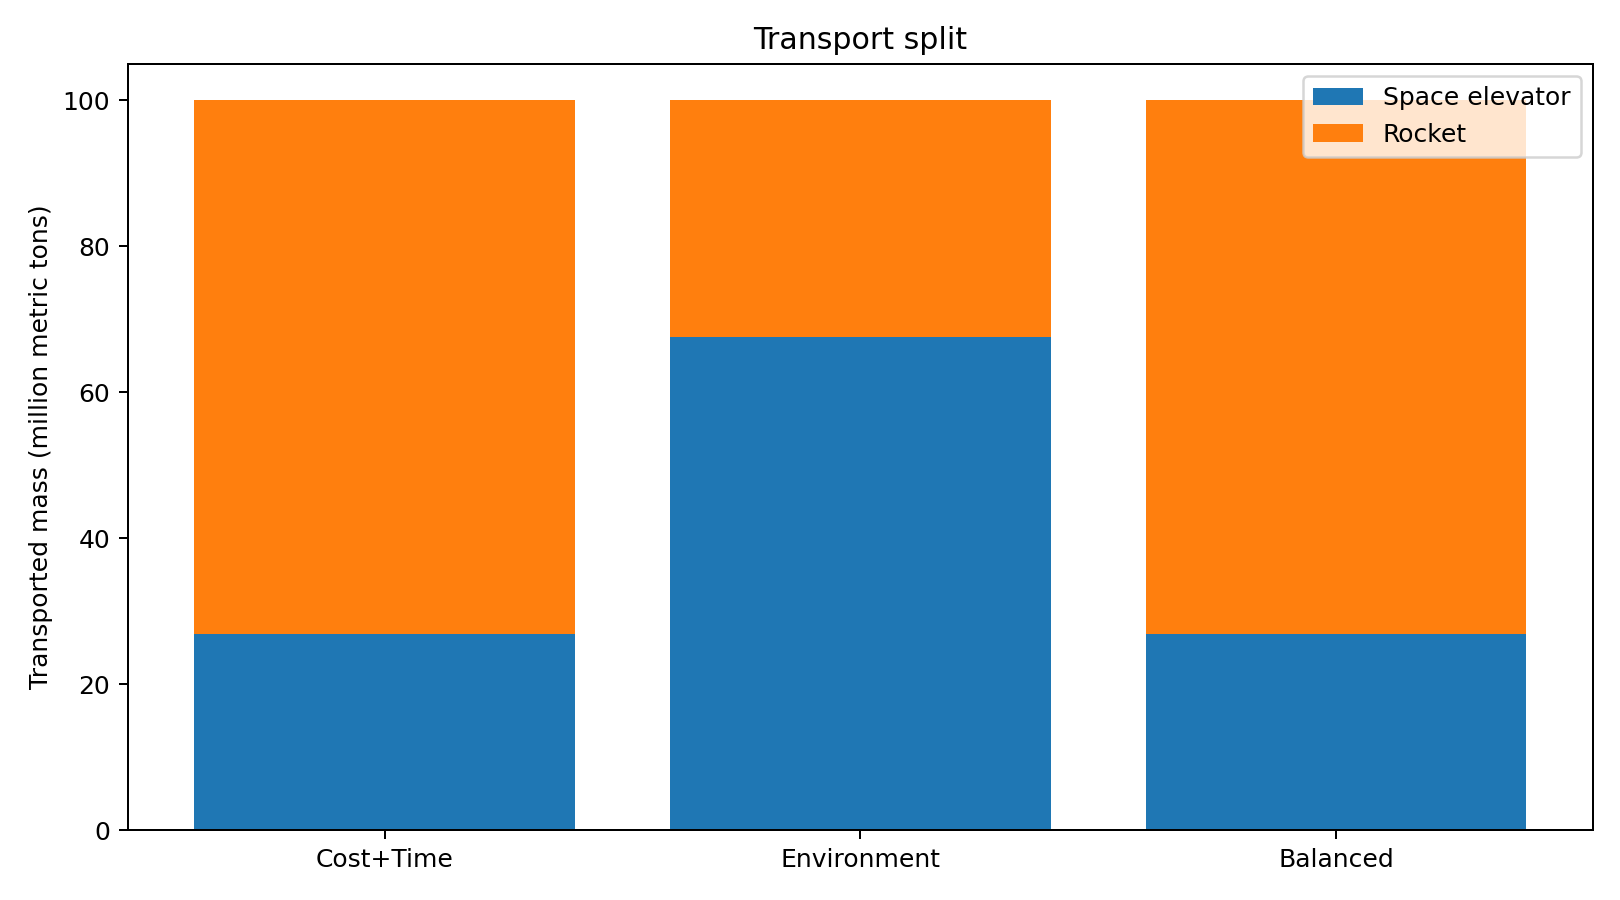
\includegraphics[width=\textwidth]{figures/transport_split.png}
        \caption{运输量分配}
    \end{subfigure}
    \hfill
    \begin{subfigure}{0.48\textwidth}
        \centering
        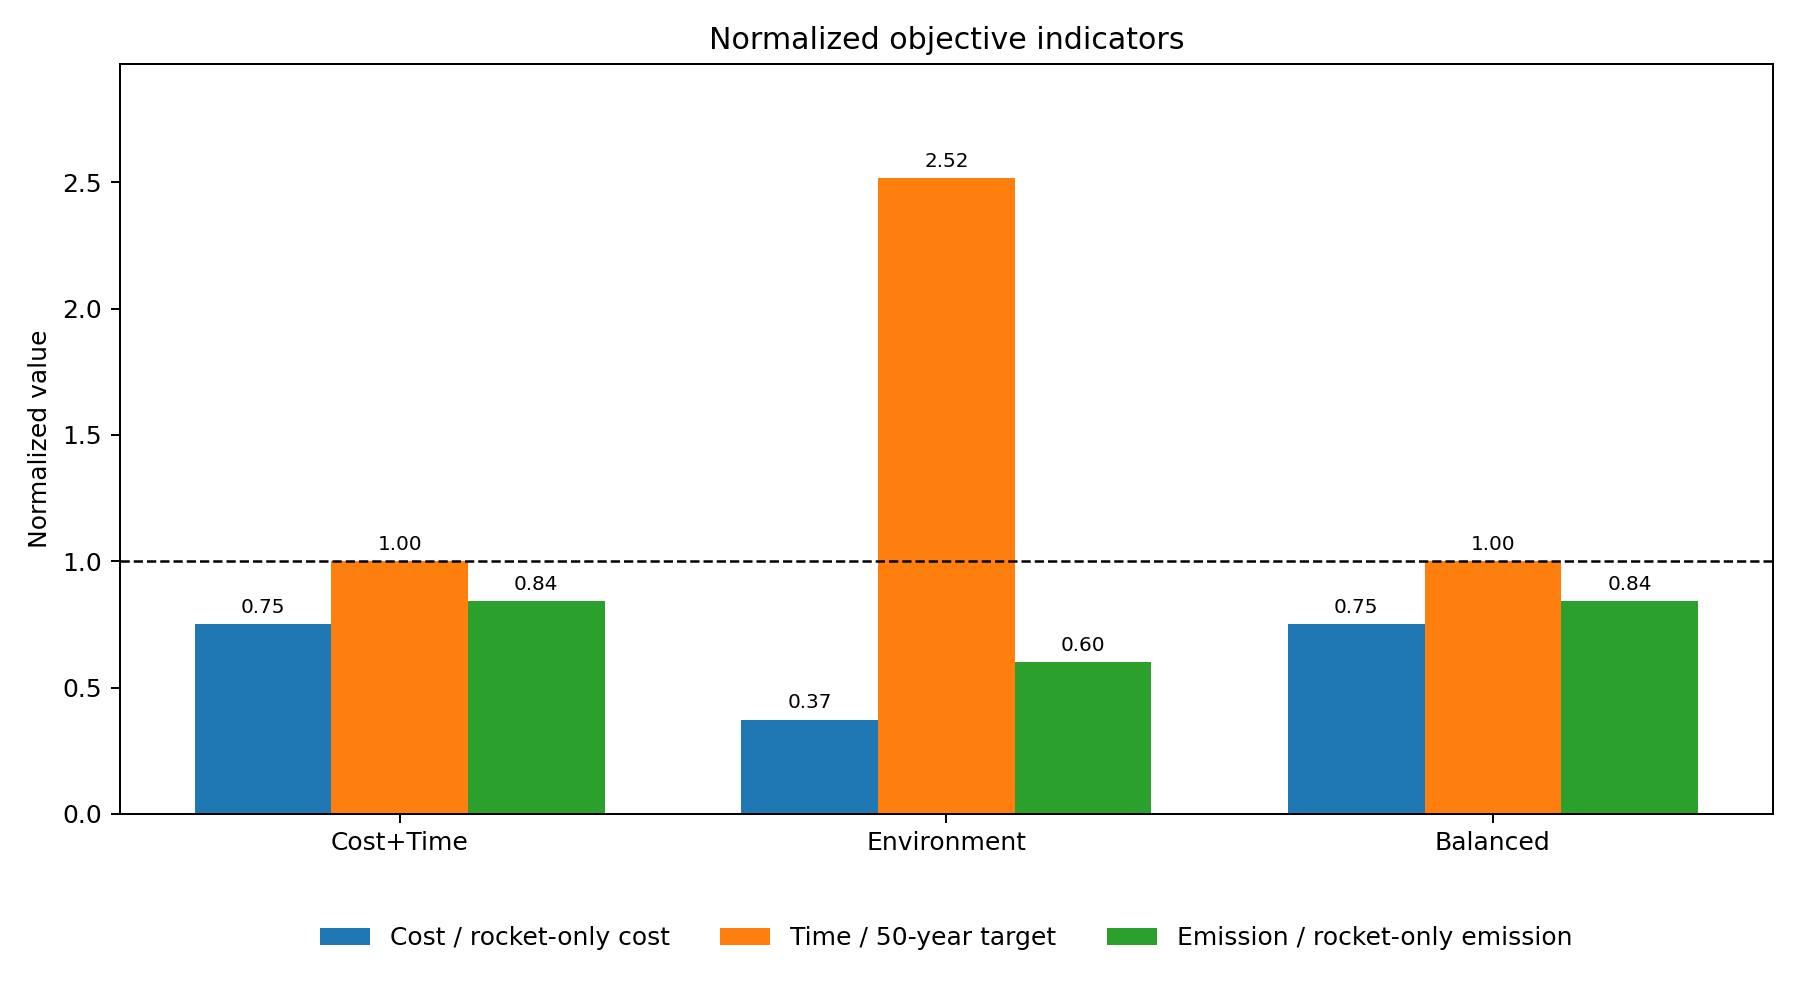
\includegraphics[width=\textwidth]{figures/normalized_metrics.png}
        \caption{归一化指标}
    \end{subfigure}
    \caption{完美工作状态下三种权重情景对比}
\end{figure}

\begin{figure}[H]
    \centering
    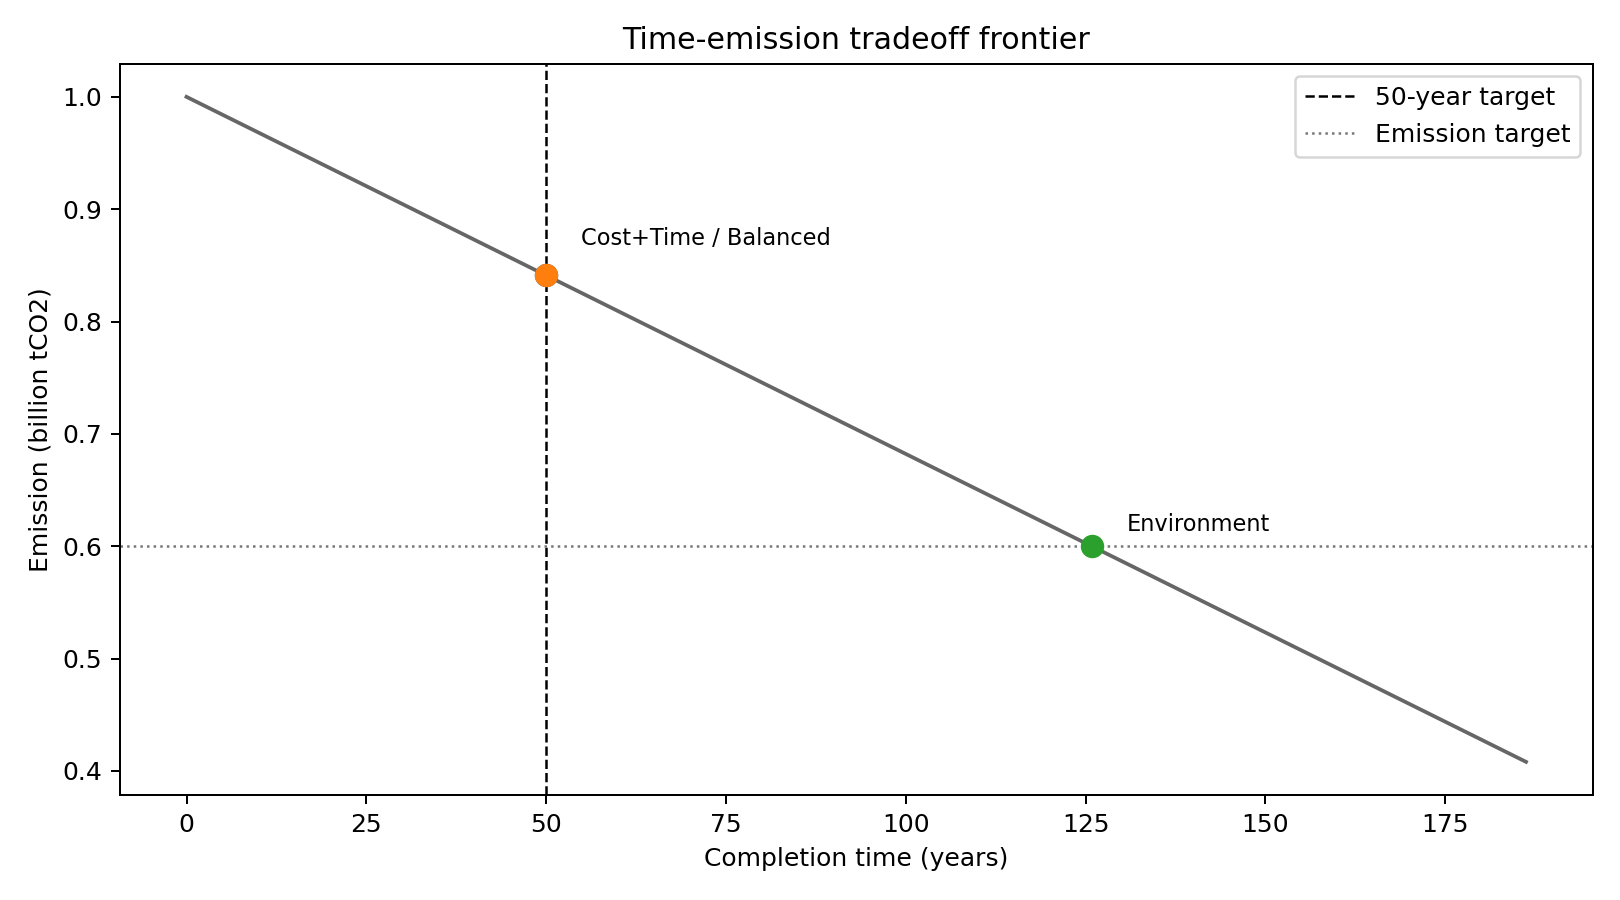
\includegraphics[width=0.72\textwidth]{figures/tradeoff_time_emission.png}
    \caption{运输工期与环境排放的权衡关系}
\end{figure}

\subsection{非完美工作状态下的解变动}

在综合非完美主情景中，取 \(a_E=0.90\)、\(a_R=0.98\)，不把风险成本加入目标函数，只修正有效运力。求解结果如下。

\begin{center}
\footnotesize
\renewcommand{\arraystretch}{1.25}
\begin{tabular}{lrrrrrr}
\toprule
情景 & 电梯 Mt & 火箭 Mt & 发射次数 & 工期/年 & 成本/TUSD & 排放/BtCO2 \\
\midrule
成本+工期优先 & 24.165 & 75.835 & 619062 & 50.00 & 112.610 & 0.872 \\
环境优先 & 68.648 & 31.352 & 255931 & 142.04 & 52.421 & 0.600 \\
均衡 & 24.165 & 75.835 & 619061 & 50.00 & 112.609 & 0.872 \\
\bottomrule
\end{tabular}
\end{center}

与完美工作状态相比，成本+工期优先和均衡情景中，电梯有效运力下降使 50 年内可由电梯承担的运输量减少约 \(10\%\)，火箭发射次数增加约 \(5.79\%\)，总成本增加约 \(5.39\%\)，排放增加约 \(3.73\%\)。环境优先情景为了保持排放目标，进一步延长工期到 \(142.04\) 年，说明环境优先方案对电梯可用率更加敏感。

\begin{figure}[H]
    \centering
    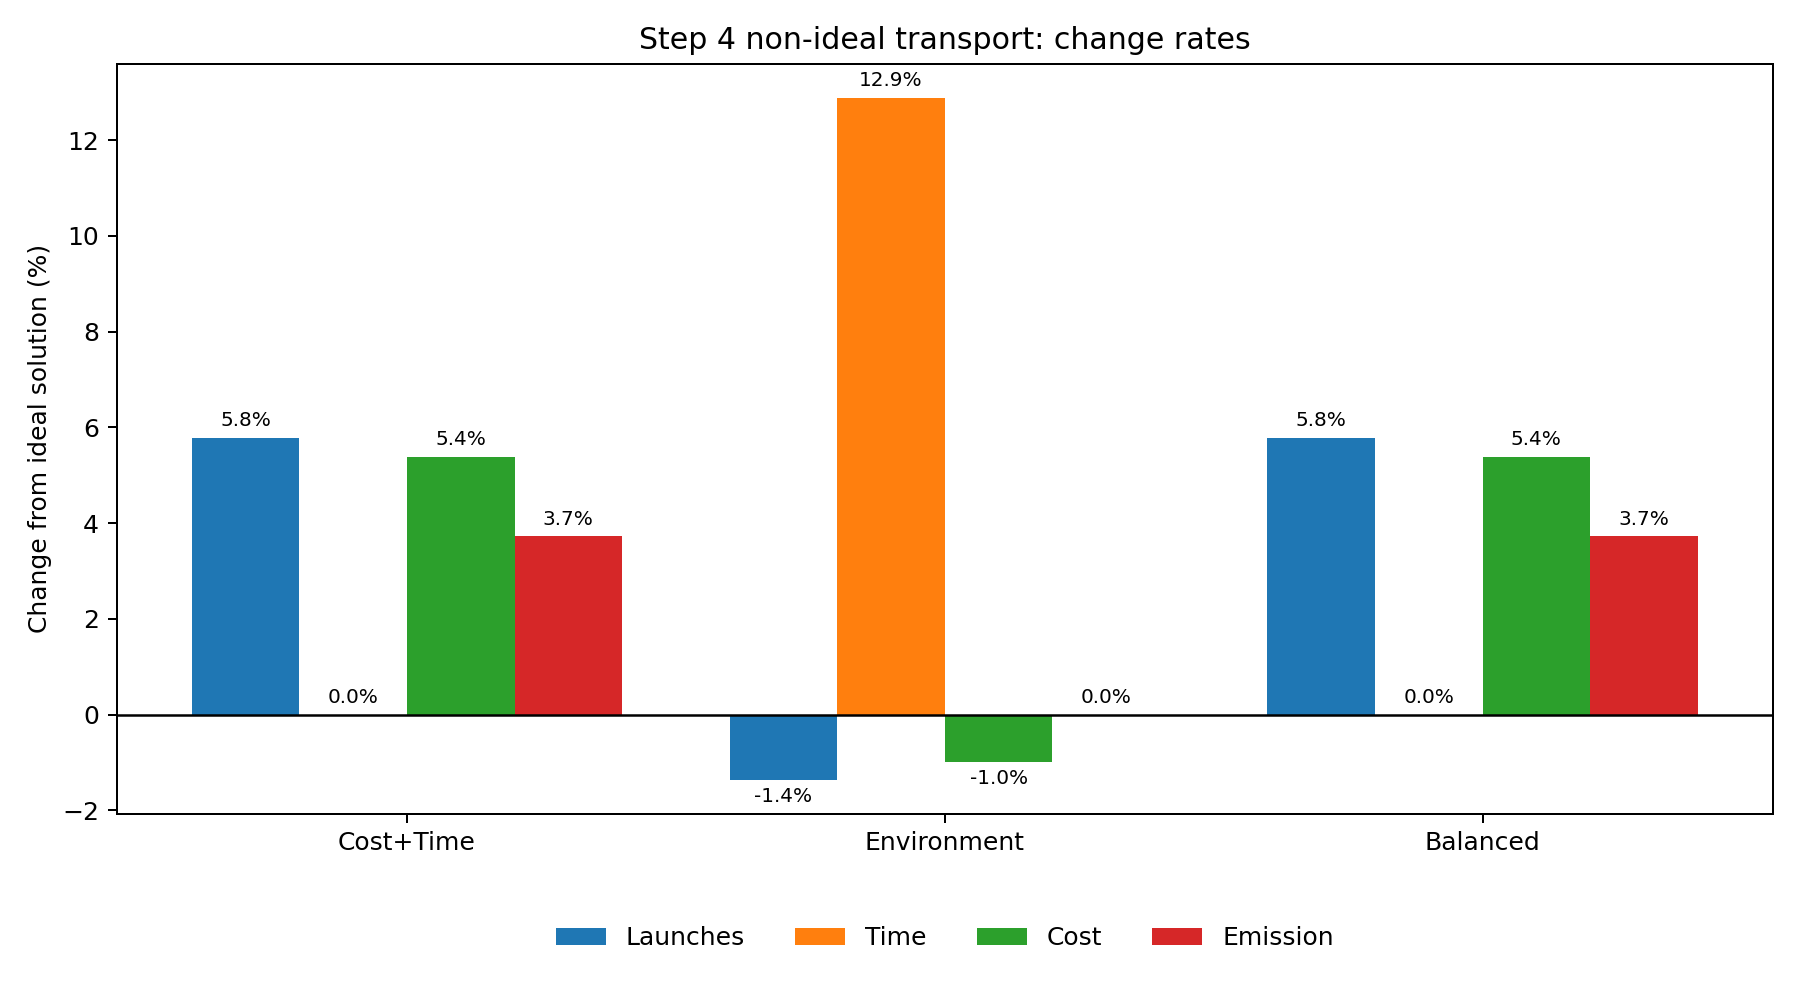
\includegraphics[width=0.76\textwidth]{figures/nonideal_change_rates.png}
    \caption{非完美工作状态相对完美工作状态的变化率}
\end{figure}

\subsection{扩展模型结果}

扩展模型同时考虑发射场环境敏感性、连续高频发射的非线性环境累积影响、10/60/30 建设运输节奏和火箭技术进步。该模型不设置月球基地最大接收能力，也不设置单个发射场的硬性年发射上限，而是通过环境损害目标引导发射场和年份分配。

\begin{center}
\footnotesize
\renewcommand{\arraystretch}{1.25}
\begin{tabular}{lrrrrrrr}
\toprule
情景 & 最优工期 & 电梯 Mt & 火箭 Mt & 发射次数 & 成本/TUSD & CO2/Bt & 环境损害 \\
\midrule
成本+工期优先 & 75 & 36.247 & 63.753 & 520430 & 75.786 & 0.708 & 0.785 \\
环境优先 & 116 & 54.947 & 45.053 & 367782 & 50.625 & 0.592 & 0.600 \\
均衡 & 79 & 38.180 & 61.820 & 504649 & 74.295 & 0.701 & 0.738 \\
\bottomrule
\end{tabular}
\end{center}

扩展模型的结果与基础模型相比更符合长期工程直觉。由于火箭成本和排放随时间下降，同时施工节奏要求前期、中期、后期按 10/60/30 运送，模型不再简单地把工期压在 50 年，而是在不同目标偏好下选择更长的建设周期。成本+工期优先情景选择 75 年；环境优先情景选择 116 年；均衡情景选择 79 年，位于 \(75\) 到 \(90\) 年之间。

\begin{figure}[H]
    \centering
    \captionsetup{skip=2pt}
    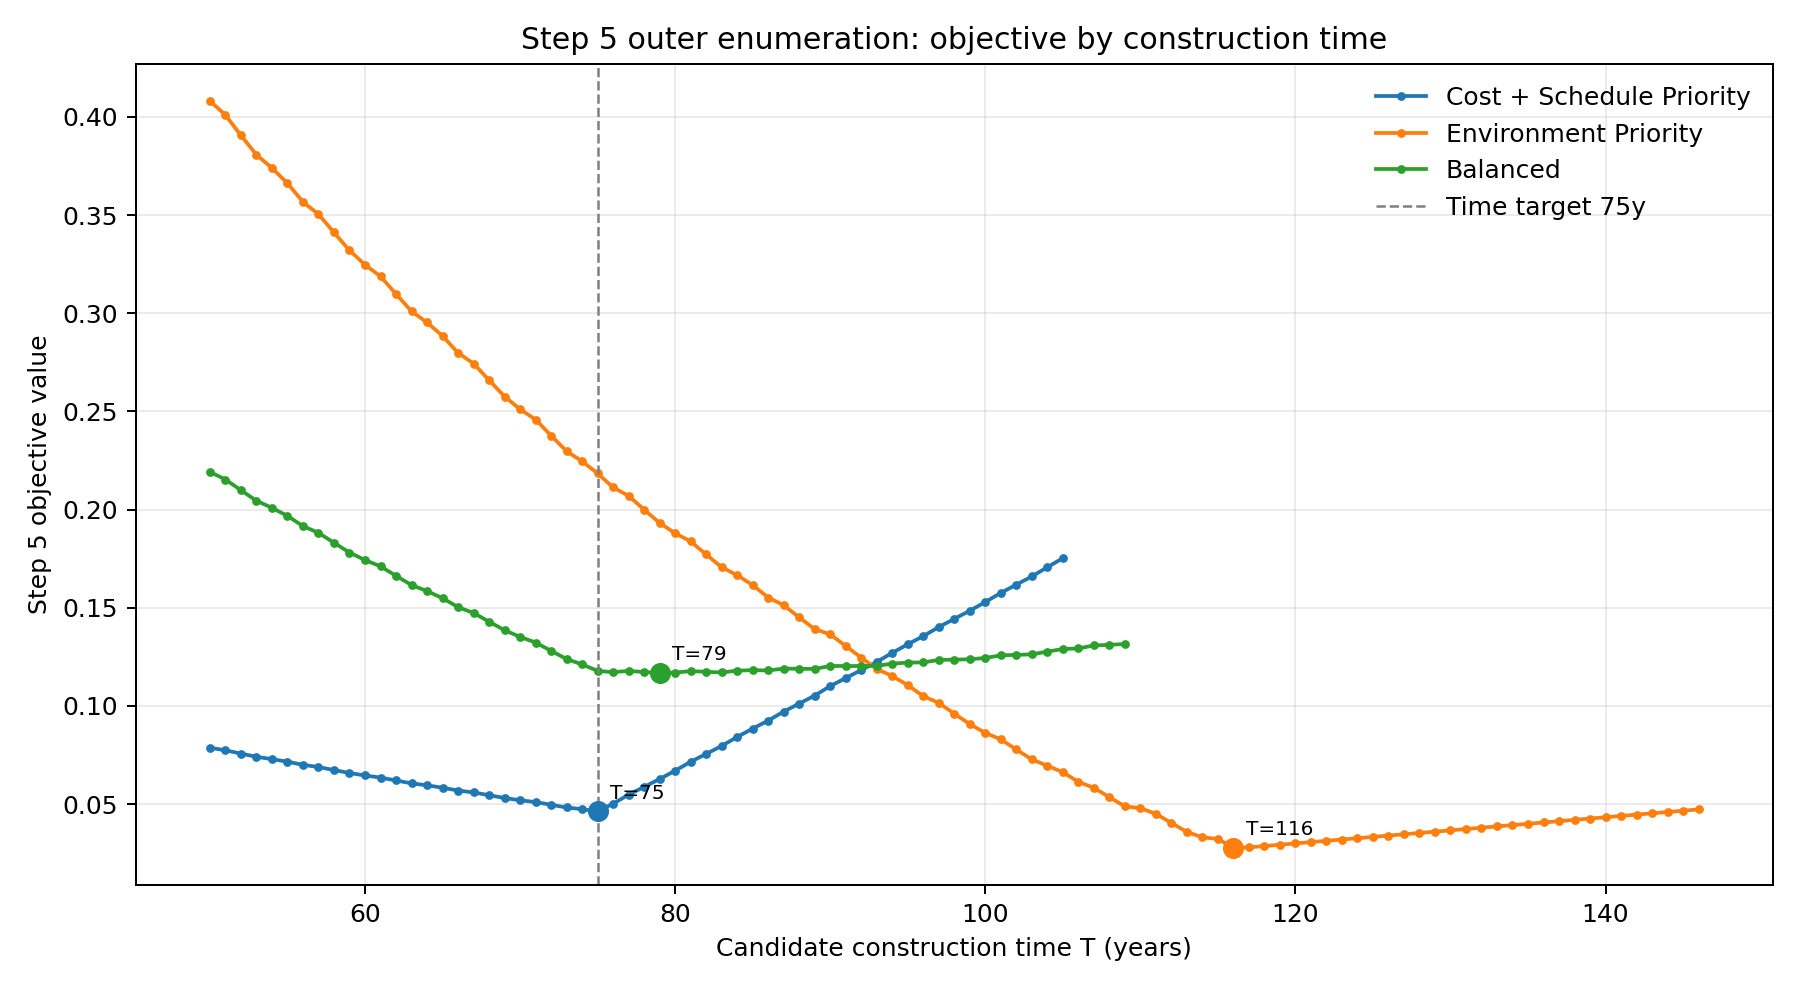
\includegraphics[width=0.88\textwidth]{figures/extended_objective_by_time.png}
    \caption{扩展模型候选工期目标函数}
\end{figure}

\begin{figure}[H]
    \centering
    \captionsetup{skip=2pt}
    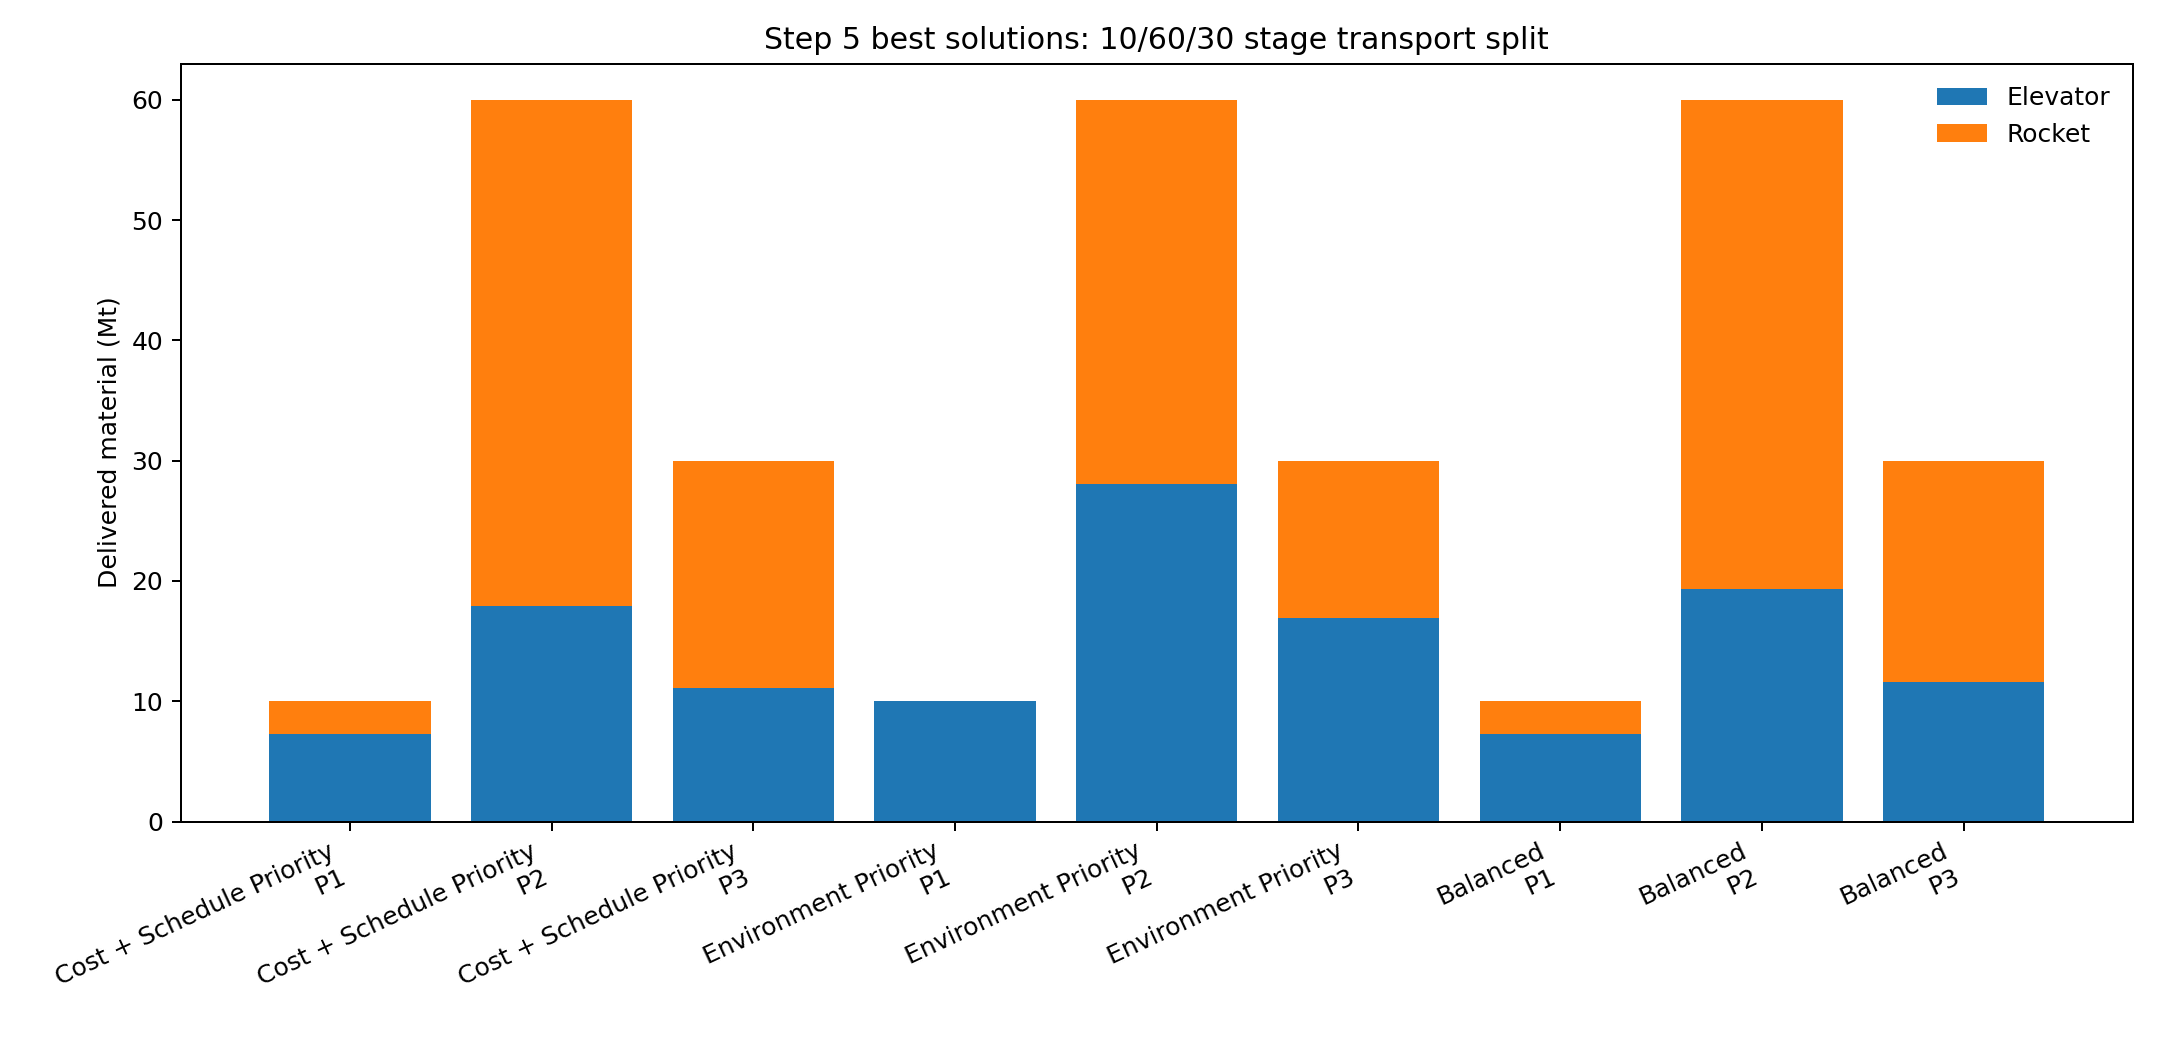
\includegraphics[width=0.88\textwidth]{figures/extended_stage_transport.png}
    \caption{扩展模型 10/60/30 阶段运输结果}
\end{figure}

\begin{figure}[H]
    \centering
    \captionsetup{skip=2pt}
    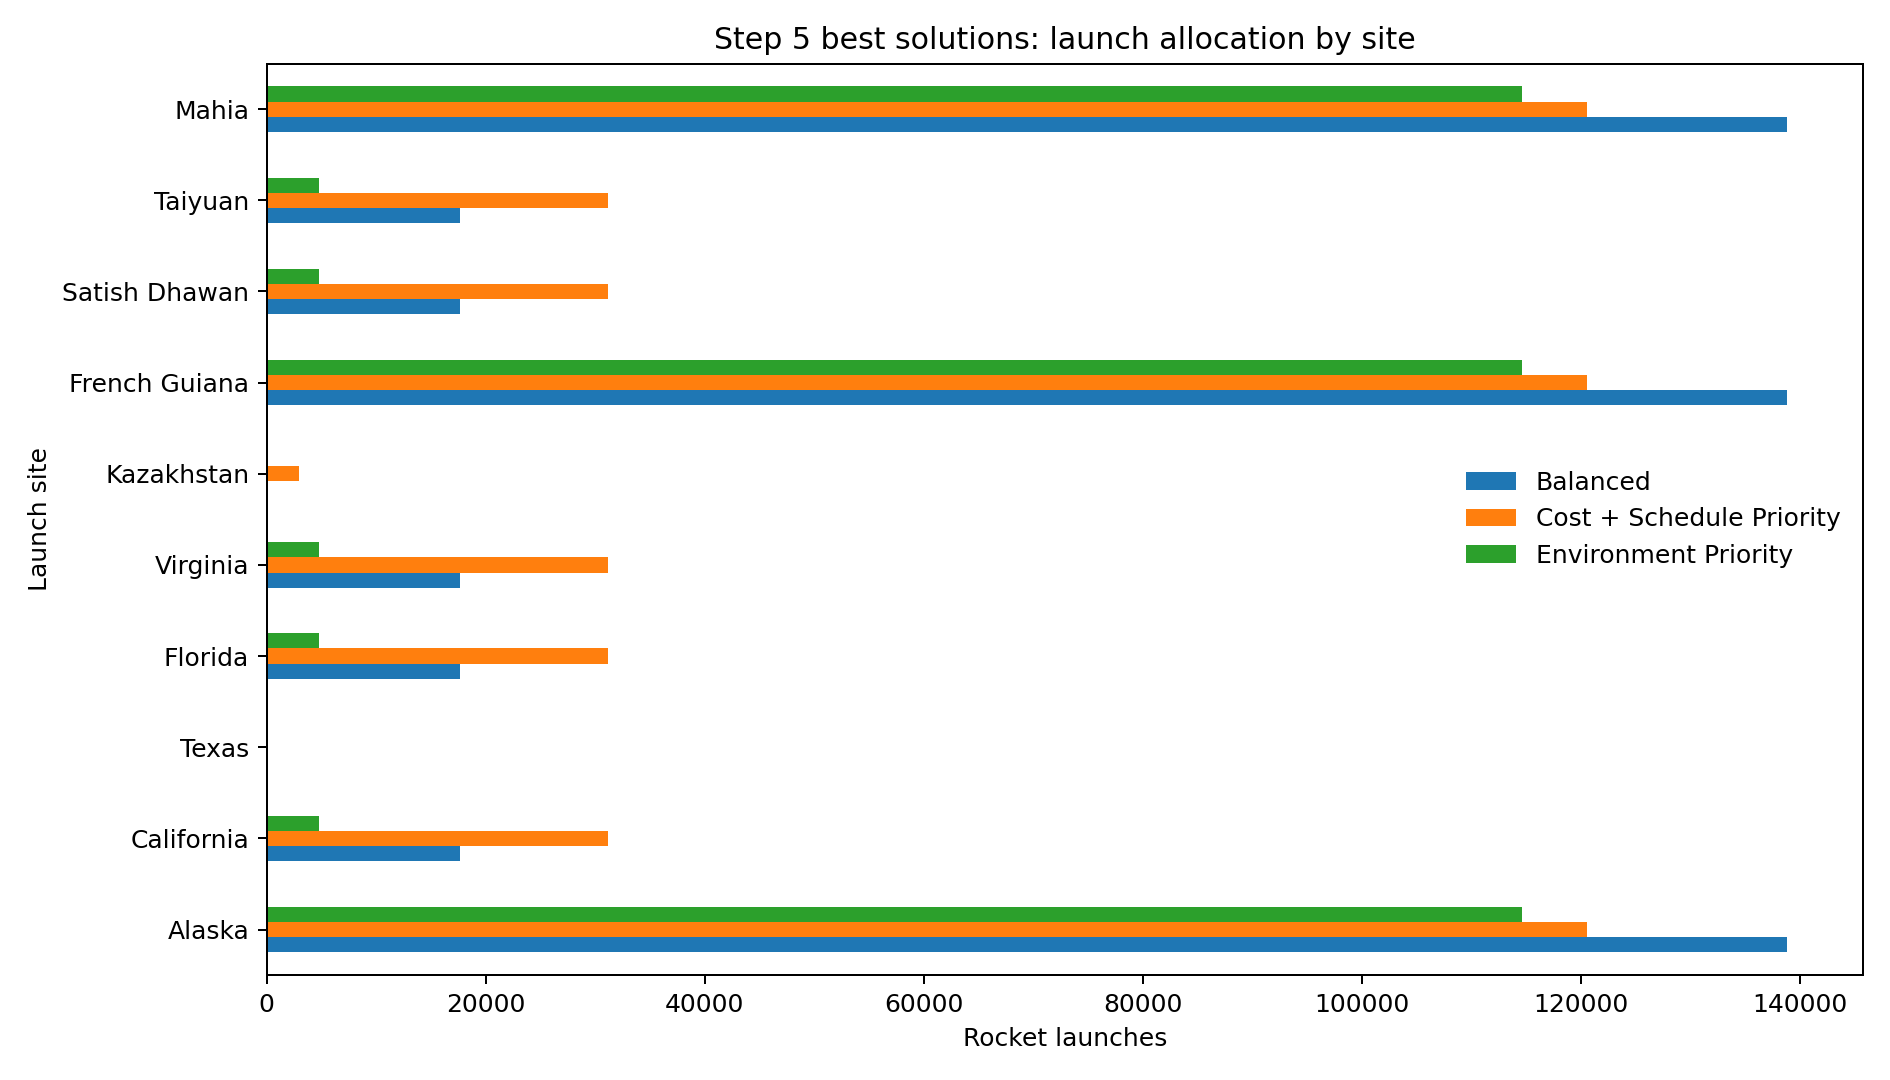
\includegraphics[width=0.88\textwidth]{figures/extended_site_launches.png}
    \caption{扩展模型中的发射场分配}
\end{figure}

\subsection{解的评估}

从成本角度看，混合运输方案明显优于纯火箭方案。基础模型中成本+工期优先方案成本为 \(106.851\) trillion USD，相比纯火箭方案 \(142.40\) trillion USD 降低约 \(24.96\%\)。扩展模型中，由于考虑火箭技术进步，成本+工期优先方案进一步降至 \(75.786\) trillion USD，均衡方案为 \(74.295\) trillion USD。

从工期角度看，纯电梯方案不可接受，纯火箭方案虽然可以压缩工期但代价过高。基础混合模型能在 50 年内完成，但需要大量火箭发射；扩展模型放宽为长期建设后，能够在 75--79 年附近取得更平衡的方案。

从环境角度看，环境优先方案显著降低火箭运输量。基础模型中环境优先方案排放为 \(0.600\) billion tCO2，约为纯火箭方案的 \(60\%\)；扩展模型中环境优先方案物理 CO2 排放约为 \(0.592\) billion tCO2，并通过发射场分散调度降低综合环境损害。

从稳定性角度看，非完美工作状态不会推翻混合运输的基本结论，但会提高火箭补充需求。若坚持 50 年完成，电梯可用率下降必须由更多火箭发射补足；若更重视环境，则系统会主动延长工期以降低火箭使用强度。

\subsection{方法对比}

本文共比较了四类方法。

第一，极端方案计算方法简单直观，适合作为 benchmark，但不能直接给出推荐方案。

第二，HiGHS 混合整数目标规划能够完整表达约束和目标，具有标准运筹学模型形式，是本文的主求解方法。

第三，一维整数搜索利用了基础模型的特殊结构，结果与 HiGHS MILP 的最大差异约为 \(1.56\times10^{-13}\)，说明该方法可以作为可靠校验，并可快速生成权衡曲线。

第四，扩展模型的外层枚举和内层凸二次调度近似牺牲了一定精确性，但换来了更强的解释性，可以处理发射场级环境敏感性、非线性累积影响和技术进步。对于课程作业而言，这种“标准模型 + 可解释近似”的方法比直接堆叠复杂黑箱求解更容易说明模型含义。

\clearpage
\section{结论}

\subsection{研究结论}

本文围绕月球基地建设期 \(100\) Mt 材料运输问题，建立了从基础目标规划到扩展多时期调度的第一阶段模型，并得出以下结论。

第一，单一运输方式都不是合理最终方案。纯太空电梯方案成本和排放较低，但需要约 \(186.22\) 年；纯火箭方案需要 \(800000\) 次发射，成本和排放过高。因此，应采用太空电梯和火箭结合的混合运输方案。

第二，在完美工作状态下，若强调成本和工期，推荐 50 年完成的混合运输结构：太空电梯运输 \(26.850\) Mt，火箭运输 \(73.150\) Mt，火箭发射 \(585200\) 次，总成本约 \(106.851\) trillion USD，总排放约 \(0.841\) billion tCO2。若环境优先，则应显著增加电梯承担比例，但工期将延长到约 \(125.82\) 年。

第三，非完美工作状态主要表现为火箭补偿需求上升。在 \(a_E=0.90,a_R=0.98\) 情景下，成本+工期优先方案仍保持 50 年完成，但火箭发射次数增加到 \(619062\) 次，成本和排放分别上升约 \(5.39\%\) 和 \(3.73\%\)。

第四，扩展模型表明，长期建设情景下不必机械追求 50 年完成。考虑发射场环境敏感性、连续发射非线性环境压力、10/60/30 施工节奏和技术进步后，成本+工期优先方案选择 75 年，均衡方案选择 79 年，环境优先方案选择 116 年。该结果说明，适当拉长建设周期可以显著降低火箭发射压力、运输成本和环境损害。

综合考虑可解释性、成本、工期和环境影响，本文推荐以扩展模型中的均衡方案作为课程报告的主要建议方案：在约 79 年内完成运输，太空电梯承担 \(38.180\) Mt，火箭承担 \(61.820\) Mt，火箭发射约 \(504649\) 次，总成本约 \(74.295\) trillion USD，物理 CO2 排放约 \(0.701\) billion tCO2。该方案没有最低环境方案那么慢，也比基础 50 年方案更能体现长期工程中的成本下降和环境约束。

\subsection{亮点与心得}

本报告的主要亮点在于：没有直接把题目处理成一次简单代入计算，而是按运筹学思想逐步抽象。我们先建立极端方案基准，再用目标规划处理多目标冲突，随后用非完美工作状态检验方案稳定性，最后扩展到发射场级调度与非线性环境影响。

完成本次大作业的收获主要有三点。第一，目标规划适合处理“没有唯一绝对最优”的工程决策问题，权重和目标值本身就是决策偏好的数学表达。第二，模型不一定越复杂越好，先写出可解释的基础模型，再逐步加入现实因素，更有利于分析结果变化。第三，运筹学建模不仅是求一个数值答案，更重要的是说明不同约束、目标和假设如何改变决策结论。

\clearpage
\section{参考文献}
\label{sec:references}

\begingroup
\footnotesize
\raggedright
\sloppy
\begin{enumerate}
    \item[{[1]}] COMAP. \textit{Creating a Moon Colony Using a Space Elevator System: 2026 MCM Problem B}. Available: \url{https://www.comap.org/membership/member-resources/item/creating-a-moon-colony-using-a-space-elevator-system}.
    \item[{[2]}] Raitt, D. and Edwards, B. C. \textit{The Space Elevator: Economics and Applications}. International Astronautical Congress, 2004. Available: \url{https://media2.spaceref.com/docs/spaceelevator/iac-2004/iac-04-iaa.3.8.3.09.raitt.pdf}.
    \item[{[3]}] Edwards, B. C. \textit{The Space Elevator}. NASA Goddard Colloquium Archive, 2003. Available: \url{https://ecolloq.gsfc.nasa.gov/archive/2003-Fall/announce.edwards.html}.
    \item[{[4]}] Edwards, B. C. \textit{The Space Elevator: NIAC Phase II Final Report}. NASA Institute for Advanced Concepts, 2003. Available: \url{https://www.niac.usra.edu/files/studies/final_report/521Edwards.pdf}.
    \item[{[5]}] Intergovernmental Panel on Climate Change. \textit{Climate Change 2014: Mitigation of Climate Change, Annex III}. Available: \url{https://www.ipcc.ch/site/assets/uploads/2018/02/ipcc_wg3_ar5_annex-iii.pdf}.
    \item[{[6]}] U.S. Environmental Protection Agency. \textit{eGRID Summary Data}. Available: \url{https://www.epa.gov/egrid/summary-data}.
    \item[{[7]}] SpaceX. \textit{Falcon Heavy}. Available: \url{https://www.spacex.com/vehicles/falcon-heavy}.
    \item[{[8]}] SpaceX. \textit{Falcon User's Guide}. Available: \url{https://www.spacex.com/assets/media/falcon-users-guide-2025-05-09.pdf}.
    \item[{[9]}] NASA. \textit{NASA Awards Launch Services Contract for Europa Clipper Mission}. Available: \url{https://www.nasa.gov/news-release/nasa-awards-launch-services-contract-for-europa-clipper-mission/}.
    \item[{[10]}] Federal Aviation Administration. \textit{Final Environmental Assessment and Finding of No Significant Impact for SpaceX Falcon Program}. Available: \url{https://www.faa.gov/sites/faa.gov/files/space/environmental/nepa_docs/SpaceX_Falcon_Program_Final_EA_and_FONSI.pdf}.
    \item[{[11]}] Maloney, C. M. et al. The climate and ozone impacts of black carbon emissions from global rocket launches. \textit{Journal of Geophysical Research: Atmospheres}, 2022. Available: \url{https://agupubs.onlinelibrary.wiley.com/doi/full/10.1029/2021JD036373}.
    \item[{[12]}] NASA. \textit{Moonbase: About}. Available: \url{https://www.nasa.gov/reference/moonbase-about/}.
    \item[{[13]}] NASA. \textit{Work Underway on Large Cargo Landers for NASA's Artemis Moon Missions}. Available: \url{https://www.nasa.gov/humans-in-space/work-underway-on-large-cargo-landers-for-nasas-artemis-moon-missions/}.
    \item[{[14]}] Saaty, R. W. The analytic hierarchy process: what it is and how it is used. \textit{Mathematical Modelling}, 1987. DOI: \url{https://doi.org/10.1016/0270-0255(87)90473-8}.
    \item[{[15]}] UK HM Treasury. \textit{Green Book Supplementary Guidance: Multi-Criteria Decision Analysis}. Available: \url{https://www.gov.uk/government/publications/green-book-supplementary-guidance-multi-criteria-decision-analysis}.
\end{enumerate}
\endgroup

\clearpage
\section{附录}
\label{app:appendix}

\subsection{补充参数表}
\label{app:params}

正文没有展开的参数主要用于环境排放推算、发射场级调度和扩展模型。

\begin{center}
\footnotesize
\renewcommand{\arraystretch}{1.22}
\begin{tabular}{p{0.16\textwidth}p{0.47\textwidth}p{0.27\textwidth}}
\toprule
符号 & 含义 & 本文取值或口径 \\
\midrule
\(e_E\) & 太空电梯单位运输用电量 & \(85000\) kWh/公吨 \\
\(\gamma_E\) & 电梯用电排放因子 & 太阳能生命周期排放 \(0.048\) kgCO2e/kWh \\
\(g_E\) & 太空电梯单位运输排放 & \(e_E\gamma_E/1000=4.08\) tCO2/公吨 \\
\(\tau_R\) & 火箭燃料类型 & Falcon Heavy 使用 LOX/RP-1 \\
\(a_E\) & 太空电梯系统可用率 & 主情景 \(0.90\) \\
\(a_R\) & 火箭有效交付率 & 主情景 \(0.98\) \\
\(\lambda_f\) & 火箭发射成本年下降率 & \(0.5\%\) \\
\(\lambda_g\) & 火箭单次排放年下降率 & \(0.3\%\) \\
\(\beta\) & 非线性环境压力系数 & \(2.5\times10^{-11}\) \\
\bottomrule
\end{tabular}
\end{center}

\subsection{发射场位置与环境敏感系数}
\label{app:sites}

\begin{center}
\footnotesize
\renewcommand{\arraystretch}{1.18}
\begin{tabular}{p{0.23\textwidth}p{0.30\textwidth}cc}
\toprule
发射场 & 位置口径 & 环境敏感系数 \(s_i\) & 延误率 \(\delta_i\) \\
\midrule
Alaska & Kodiak/Narrow Cape, \(57.43^\circ\)N, \(152.34^\circ\)W & 3.5 & 0.20 \\
California & Vandenberg SFB, \(34.58^\circ\)N, \(120.63^\circ\)W & 4.0 & 0.12 \\
Texas & Starbase/Boca Chica, \(25.99^\circ\)N, \(97.16^\circ\)W & 5.0 & 0.25 \\
Florida & KSC/Cape Canaveral, \(28.57^\circ\)N, \(80.65^\circ\)W & 4.0 & 0.28 \\
Virginia & Wallops/MARS, \(37.83^\circ\)N, \(75.48^\circ\)W & 4.0 & 0.18 \\
Kazakhstan & Baikonur, \(45.95^\circ\)N, \(63.30^\circ\)E & 4.5 & 0.10 \\
French Guiana & Kourou, \(5.23^\circ\)N, \(52.77^\circ\)W & 3.5 & 0.15 \\
Satish Dhawan & Sriharikota, \(13.73^\circ\)N, \(80.23^\circ\)E & 4.0 & 0.18 \\
Taiyuan & Taiyuan Satellite Launch Center, \(38.85^\circ\)N, \(111.61^\circ\)E & 4.0 & 0.10 \\
Mahia & Rocket Lab LC-1, \(39.26^\circ\)S, \(177.86^\circ\)E & 3.5 & 0.20 \\
\bottomrule
\end{tabular}
\end{center}

其中 \(s_i\) 越大表示环境敏感性越强。Texas 因生态和社区争议取最高；Kazakhstan 因历史推进剂和落区污染风险取较高；Alaska、French Guiana 和 Mahia 因相对偏远或近海开阔取较低。

\subsection{步骤 4 次核心代码}
\label{app:code-nonideal}

\begin{lstlisting}[language=Python]
def evaluate_nonideal(n_launches, weights):
    x_rocket = a_r * rocket_payload * n_launches
    x_elevator = max(0.0, material_demand - x_rocket)
    time = x_elevator / (a_e * elevator_capacity)
    cost = elevator_cost * x_elevator + rocket_cost * n_launches
    emission = elevator_emission * x_elevator + rocket_emission * n_launches
    return goal_value(cost, time, emission, weights)
\end{lstlisting}

\subsection{步骤 5 内层调度次核心代码}
\label{app:code-step5}

\begin{lstlisting}[language=Python]
def allocate_convex_integer(total, linear, quad):
    # Minimize sum linear*x + quad*x^2
    # subject to integer x >= 0 and sum x = total.
    low = float(linear.min())
    high = float((linear + 2.0 * quad * total).max())
    for _ in range(90):
        mu = 0.5 * (low + high)
        x = np.maximum(0.0, (mu - linear) / (2.0 * quad))
        if x.sum() < total:
            low = mu
        else:
            high = mu
    base = np.floor(np.maximum(0.0, (high - linear) / (2.0 * quad)))
    return repair_to_integer_total(base, total)
\end{lstlisting}

\subsection{结果文件索引}

\begin{itemize}
    \item \texttt{result/mixed\_model\_results.md}：步骤 1--3 基础模型结果。
    \item \texttt{result/reduced\_search\_results.md}：一维整数搜索结果。
    \item \texttt{result/nonideal\_results.md}：步骤 4 非完美工作状态结果。
    \item \texttt{result/extended\_model\_results.md}：步骤 5 扩展模型结果。
    \item \texttt{report/figures/}：报告中使用的所有可视化图表。
\end{itemize}

\section{分工与贡献}

\begin{center}
\small
\renewcommand{\arraystretch}{1.25}
\begin{tabular}{p{0.13\textwidth}p{0.31\textwidth}p{0.45\textwidth}}
\toprule
成员 & 主要负责内容 & 具体贡献 \\
\midrule
曹航硕 & 基础目标规划建模；太空电梯相关数据调查 & 负责完美工作状态模型中的基础运输结构与三目标规划部分，参与建立成本、工期、环境目标函数；调查太空电梯单位运输成本、运输耗电量和电力排放因子，并整理对应来源与推算口径。 \\
吴天昊 & 火箭运输参数建模；火箭相关数据调查 & 负责完美工作状态模型中的火箭运输 benchmark 与火箭发射次数整数约束部分；调查火箭单次载荷、发射成本、推进剂和单次发射 CO2 排放等参数，并参与核验 NASA 与 SpaceX 相关来源。 \\
陈禹成 & 非完美工作状态模型；发射场数据调查 & 负责非完美工作状态模型中的可用率修正部分，建立 \(a_E,a_R\) 对有效运力的约束修正；调查发射场位置、延误率和环境敏感性系数，为扩展模型提供发射场级参数。 \\
邓凯坤 & 混合整数规划求解代码 & 负责 \texttt{solve\_mixed\_model.py} 的核心求解实现，使用 SciPy MILP/HiGHS 构造目标函数、偏差变量、线性约束和整数变量，并输出三组权重情景下的最优解。 \\
朱奕辰 & 降维搜索与非完美情景代码 & 负责 \texttt{solve\_reduced\_search.py} 和 \texttt{solve\_nonideal.py} 的实现，用一维整数搜索校验 MILP 结果，并计算非完美工作状态相对完美工作状态的变化率。 \\
{\CJKfontspec{Songti SC}康褀} & 扩展模型代码与可视化 & 负责 \texttt{solve\_extended\_model.py} 的外层工期枚举和内层凸二次调度近似实现，生成扩展模型的阶段运输、发射场分配和目标函数曲线等可视化图表。 \\
\bottomrule
\end{tabular}
\end{center}

\clearpage

% \appendix

% \section{附录1：}

% \begin{lstlisting}
% \end{lstlisting}


% \section{附录2：}
% \reference






\end{document}
